%%
%% This is file `sample-acmsmall.tex',
%% generated with the docstrip utility.
%%
%% The original source files were:
%%
%% samples.dtx  (with options: `acmsmall')
%% 
%% IMPORTANT NOTICE:
%% 
%% For the copyright see the source file.
%% 
%% Any modified versions of this file must be renamed
%% with new filenames distinct from sample-acmsmall.tex.
%% 
%% For distribution of the original source see the terms
%% for copying and modification in the file samples.dtx.
%% 
%% This generated file may be distributed as long as the
%% original source files, as listed above, are part of the
%% same distribution. (The sources need not necessarily be
%% in the same archive or directory.)
%%
%%
%% Commands for TeXCount
%TC:macro \cite [option:text,text]
%TC:macro \citep [option:text,text]
%TC:macro \citet [option:text,text]
%TC:envir table 0 1
%TC:envir table* 0 1
%TC:envir tabular [ignore] word
%TC:envir displaymath 0 word
%TC:envir math 0 word
%TC:envir comment 0 0
%%
%%
%% The first command in your LaTeX source must be the \documentclass
%% command.
%%
%% For submission and review of your manuscript please change the
%% command to \documentclass[manuscript, screen, review]{acmart}.
%%
%% When submitting camera ready or to TAPS, please change the command
%% to \documentclass[sigconf]{acmart} or whichever template is required
%% for your publication.
%%
%%
\documentclass[acmsmall]{acmart}

%%
%% \BibTeX command to typeset BibTeX logo in the docs
\AtBeginDocument{%
  \providecommand\BibTeX{{%
    Bib\TeX}}}

%% Rights management information.  This information is sent to you
%% when you complete the rights form.  These commands have SAMPLE
%% values in them; it is your responsibility as an author to replace
%% the commands and values with those provided to you when you
%% complete the rights form.
% \setcopyright{acmlicensed}
% \copyrightyear{2018}
% \acmYear{2018}
% \acmDOI{XXXXXXX.XXXXXXX}


%%
%% These commands are for a JOURNAL article.
% \acmJournal{JACM}
% \acmVolume{37}
% \acmNumber{4}
% % \acmArticle{111}
% \acmMonth{8}

%%
%% Submission ID.
%% Use this when submitting an article to a sponsored event. You'll
%% receive a unique submission ID from the organizers
%% of the event, and this ID should be used as the parameter to this command.
%%\acmSubmissionID{123-A56-BU3}

%%
%% For managing citations, it is recommended to use bibliography
%% files in BibTeX format.
%%
%% You can then either use BibTeX with the ACM-Reference-Format style,
%% or BibLaTeX with the acmnumeric or acmauthoryear sytles, that include
%% support for advanced citation of software artefact from the
%% biblatex-software package, also separately available on CTAN.
%%
%% Look at the sample-*-biblatex.tex files for templates showcasing
%% the biblatex styles.
%%

%%
%% The majority of ACM publications use numbered citations and
%% references.  The command \citestyle{authoryear} switches to the
%% "author year" style.
%%
%% If you are preparing content for an event
%% sponsored by ACM SIGGRAPH, you must use the "author year" style of
%% citations and references.
%% Uncommenting
%% the next command will enable that style.
%%\citestyle{acmauthoryear}


%%
%% end of the preamble, start of the body of the document source.
\begin{document}

%%
%% The "title" command has an optional parameter,
%% allowing the author to define a "short title" to be used in page headers.
\title{Dataset for LLM Static Analysis Tuning}

%%
%% The "author" command and its associated commands are used to define
%% the authors and their affiliations.
%% Of note is the shared affiliation of the first two authors, and the
%% "authornote" and "authornotemark" commands
%% used to denote shared contribution to the research.
\author{Liam Huth}
\authornote{Both authors contributed equally to this research.}
\email{huth@ualberta.ca}
\author{Zhiqi Zhou}
\authornotemark[1]
\email{pz.zhou@outlook.com}
\affiliation{
  \institution{University of Alberta}
  \streetaddress{P.O. Box 1212}
  \city{Edmonton}
  \state{Alberta}
  \country{Canada}
  \postcode{T6G 2R3}
}

% \author{Julius P. Kumquat}
% \affiliation{%
%   \institution{The Kumquat Consortium}
%   \city{New York}
%   \country{USA}}
% \email{jpkumquat@consortium.net}

%%
%% By default, the full list of authors will be used in the page
%% headers. Often, this list is too long, and will overlap
%% other information printed in the page headers. This command allows
%% the author to define a more concise list
%% of authors' names for this purpose.
\renewcommand{\shortauthors}{Liam Huth and Peter Zhou}

%%
%% The abstract is a short summary of the work to be presented in the
%% article.
\begin{abstract}
  This research paper primarily focuses on the creation of an integrated dataset to investigate its impact on the performance of Large Language Models (LLMs), specifically in the context of static analysis for software security. Recognizing a gap in the capabilities of LLMs like ChatGPT 3.5 Turbo in accurately identifying and analyzing critical software vulnerabilities such as SQL injection, command injection, and path traversal, we hypothesize that this shortfall is partly due to the lack of specialized training datasets. To test this hypothesis, we developed a comprehensive dataset encompassing these specific vulnerabilities. Our approach involved fine-tuning ChatGPT 3.5 Turbo-0613 with this dataset and comparing its performance with its original version, as well as with other advanced models such as ChatGPT-4.0 and ChatGPT-4.0-1106 Preview. The evaluation focused on the models' proficiency in vulnerability detection, tracing the source and sink of these vulnerabilities, and analyzing the output quality. Performance metrics such as precision, recall, and F1 score were employed to assess improvements. The findings of this study aim to validate whether the integration of a tailored dataset can indeed enhance the effectiveness of LLMs in static analysis tasks, thereby contributing to the broader field of AI-assisted software security. Additionally, by making this dataset open-source, we encourage community collaboration and further research in this vital area.
\end{abstract}

%%
%% The code below is generated by the tool at http://dl.acm.org/ccs.cfm.
%% Please copy and paste the code instead of the example below.
%%
\begin{CCSXML}
<ccs2012>
    <concept>
      <concept_id>10011007.10011074.10011099.10011693</concept_id>
      <concept_desc>Software and its engineering~Empirical software validation</concept_desc>
      <concept_significance>500</concept_significance>
      </concept>
  </ccs2012>
\end{CCSXML}
  
\ccsdesc[500]{Software and its engineering~Empirical software validation}

%%
%% Keywords. The author(s) should pick words that accurately describe
%% the work being presented. Separate the keywords with commas.
\keywords{Dataset, Model Fine-Tuning, Large Language Models, Static Analysis, Vulnerability Detection}

% \received{20 February 2007}
% \received[revised]{12 March 2009}
% \received[accepted]{5 June 2009}

%%
%% This command processes the author and affiliation and title
%% information and builds the first part of the formatted document.
\maketitle

\section{Introduction}
The emergence of Large Language Models (LLMs) like ChatGPT 3.5 Turbo marks a significant advancement in the field of computational research. Their application spans a wide range of disciplines, from natural language processing to intricate problem-solving, highlighting their versatility and ever-expanding knowledge base. One area where LLMs are poised to make substantial contributions is in static analysis – a crucial component of software development and security. Static analysis involves the scrutiny of code without its execution, a task where precision and accuracy are paramount.
Despite their prowess in various domains, LLMs demonstrate a noticeable shortcoming in static analysis, particularly in the detection of specific vulnerabilities such as SQL injection, command injection, and path traversal. This discrepancy between their potential and actual performance in static analysis raises important questions and necessitates a thorough investigation.

This paper posits that one key factor limiting LLMs' effectiveness in vulnerability detection could be their limited exposure to specialized datasets in this area. To test this hypothesis, we aim to curate a dedicated dataset and assess its impact on enhancing LLMs' capability in identifying and mitigating these vulnerabilities.

In summary, our research seeks to bridge the gap in LLM performance through targeted dataset curation and training. We present the following contributions:

\begin{itemize}
  \item The development and validation of a specialized dataset tailored for tuning ChatGPT 3.5 Turbo-0613 in detecting SQL injection, command injection, and path traversal vulnerabilities.
  \item A comparative study of the performance of LLMs before and after training with this dataset.
  \end{itemize}

Our research aims to not only improve LLMs in static analysis of software vulnerabilities but also contribute to AI-assisted software security discourse. Crucially, we will develop an open-source dataset, inviting community collaboration to enhance and diversify our approach. This step is fundamental in leveraging collective expertise for advancing AI applications in software security.

\section{Terminology}
To understand the scope and implications of our research, it is essential to clarify key terms used throughout this paper.

\subsection{Large Language Models (LLMs)}
These are advanced AI models designed to understand, interpret, and generate human language. They are trained on vast datasets and can perform a range of language-related tasks.

\subsection{ChatGPT 3.5 Turbo}
A specific iteration of the LLMs developed by OpenAI, known for its efficiency and enhanced language understanding capabilities.

\subsection{Static Analysis}
The process of analyzing code without executing it. It's used to identify errors, bugs, and security vulnerabilities in the software's source code.

\subsection{SQL Injection}
A type of vulnerability that allows attackers to interfere with the queries that an application makes to its database.

\subsection{Command Injection}
This vulnerability occurs when an application passes unsafe user-supplied data (commands) to a system shell.

\subsection{Path Traversal}
A security flaw that allows attackers to access files and directories that are stored outside the web root folder.

\subsection{Open-Source Dataset}
A dataset that is made publicly available for anyone to use, modify, and distribute, often used to encourage collaborative research and development.

\section{Approach}

\subsection{Overview}

We customize a dataset to optimize ChatGPT-3.5 Turbo-0613 for static analysis tasks, comparing the fine-tuned model's performance against both its original and ChatGPT-4.0 versions.

% Workflow PDF
\begin{figure}[htp] \centering{
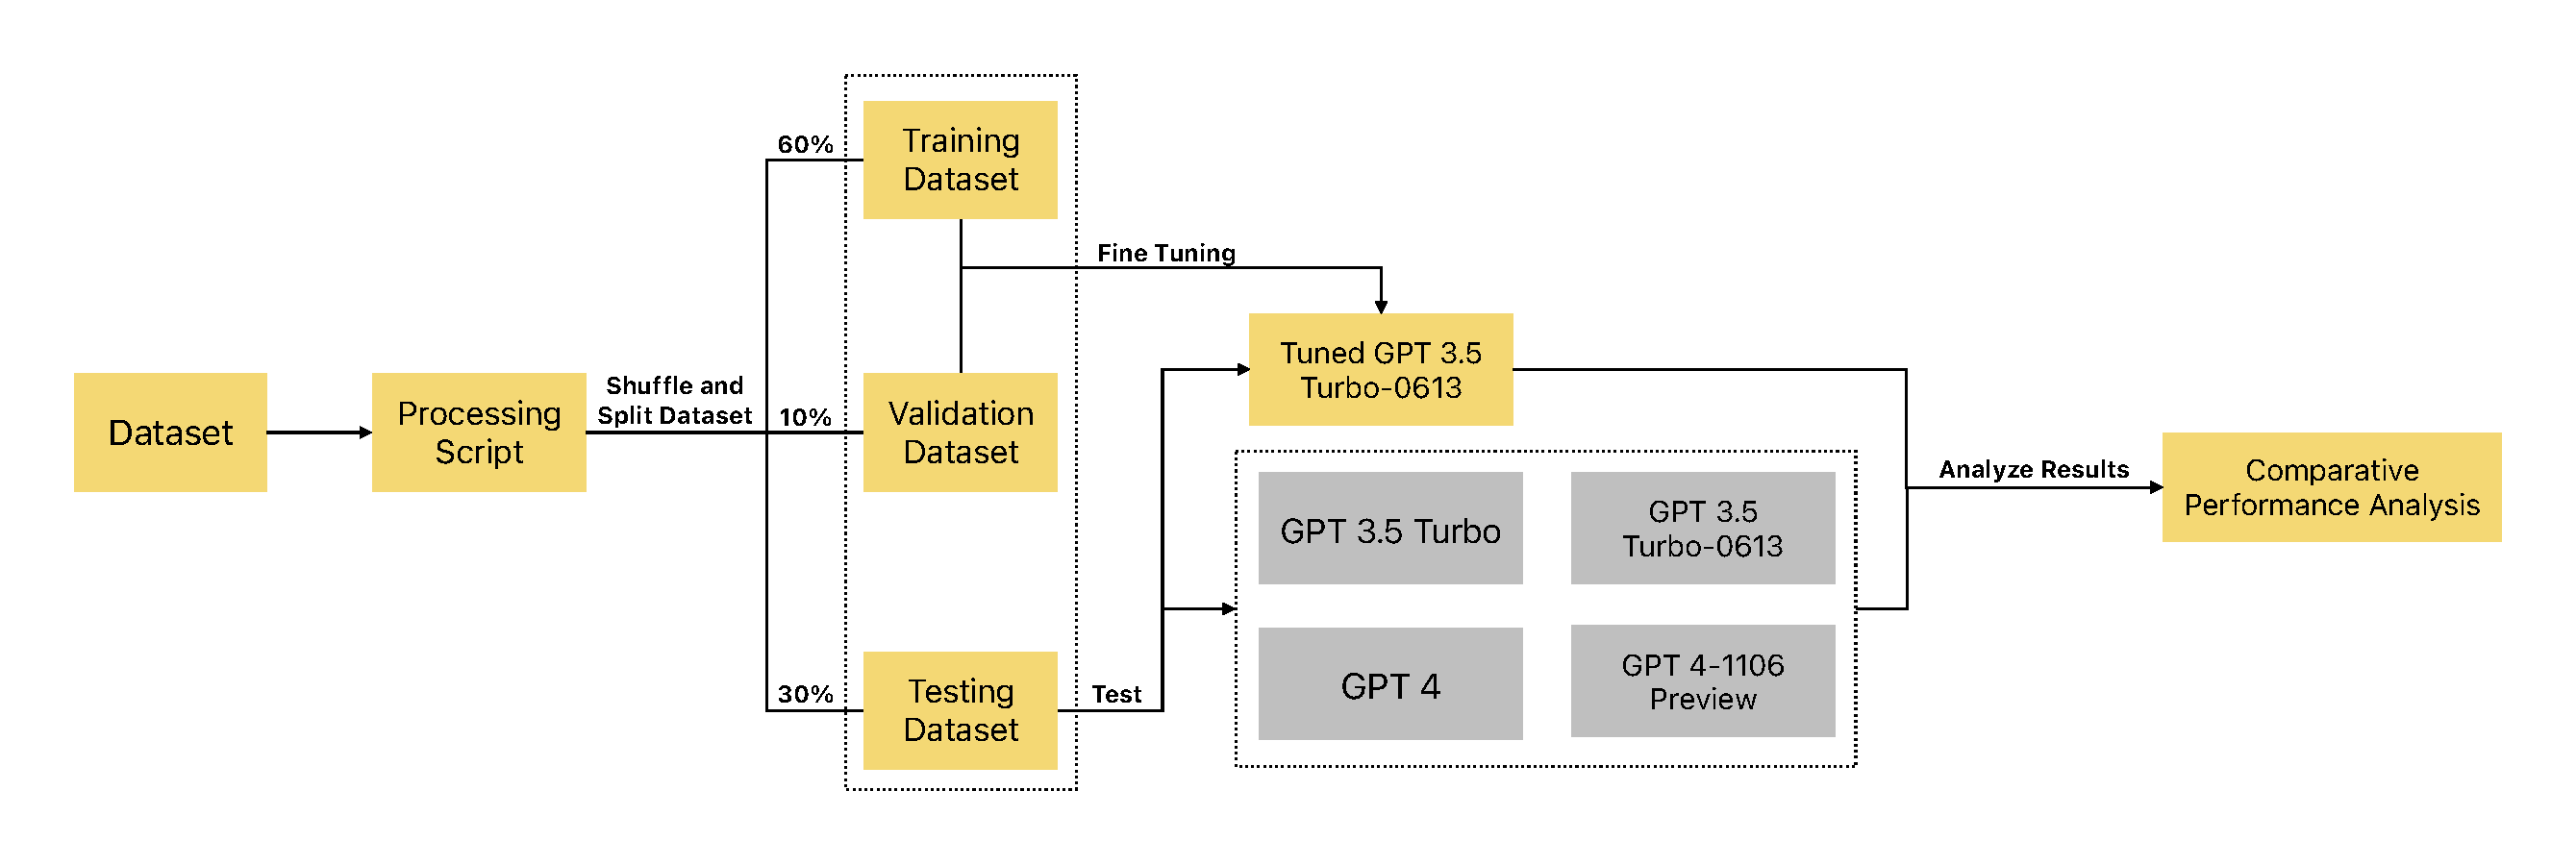
\includegraphics[scale=0.31]{../plots/workflow.pdf}}
\caption{Overview of the approach. The yellow components
are the contributions of this paper.}
\end{figure}

\subsection{Dataset Creation and Division}
\subsubsection{Dataset Composition}
Our dataset, focused on critical security vulnerabilities in software, included samples of SQL injection, path traversal, command injection, and clean code to provide a diverse range of scenarios for model training and testing.
\subsubsection{Training and Testing Split}
The dataset was divided into training, validation, and testing subsets in a 60:10:30 ratio, facilitating effective model tuning and thorough evaluation, particularly in tracing the source and sink of security vulnerabilities.

\subsection{Model Tuning and Evaluation}
\subsubsection{Fine-Tuning ChatGPT-3.5 Turbo-0613}
The fine-tuning process for ChatGPT-3.5 Turbo-0613 focused on enhancing its proficiency in identifying and tracing the source and sink of SQL injection, command injection, and path traversal vulnerabilities within code.
\subsubsection{Evaluation of Testing Dataset}
The evaluation involved comparing the performance of the fine-tuned ChatGPT-3.5 Turbo-0613, its original version, and ChatGPT-4.0, particularly in their ability to detect and analyze vulnerabilities in software.

\subsection{Comparative Performance Analysis}
\subsubsection{Output Analysis}
This phase involved analyzing the accuracy and effectiveness of the fine-tuned and original versions of ChatGPT-3.5 Turbo-0613, as well as ChatGPT-4.0 and ChatGPT-4.0-1106 Preview, in detecting vulnerabilities, with a focus on their output quality and relevance.
\subsubsection{Performance Reporting}
Our performance report detailed the improvements achieved through fine-tuning. The enhancements were measured using precision, recall, and F1 score metrics. The analysis showed significant advancements in the models' capabilities to accurately identify, trace, and report various types of vulnerabilities, their sources, and sinks. The overall findings from the report were highly positive, indicating substantial progress in all evaluated areas.


\section{Evaluation}
The following questions informed our evaluation strategy:\\
\\
Q1: How can we quantify the performance of these models on static analysis tasks?\\
Q2: What are the challenges that arise when using large language models for static analysis?\\
Q3: Are there ways we mitigate those challenges?\\
Q4: How do current state-of-the-art models perform?\\

In order to support our effort to answer these questions we ensured that our evaluation methods focused on being scalable, repeatable, and accurate. By scalable we explicitly mean that we want an increase in the size of the dataset to have minimal impact on the evaluation of the model's performance. By repeatable, we want it to be easy to control for single variables for a fine tuned analysis. Finally, we wanted to maintain the accuracy of our results despite automating the process. Will will explain later that we had to sacrifice some automation so that we could maintain accuracy.

The tools in, and the layout of, our repository are important contributions of this paper. 

Each data point consists of an input/output pair, where the input is a single source code file and the output is the expected output from the large language model. Note that while we used Python in our initial dataset, the tools we created are agnostic to the input language. This allows for arbitrary scaling of the dataset.

We include three scripts in our repository. The first, data\_formatter.py, will compile the dataset into files that can be used for training, validating, and testing the performance of OpenAI's large language models.
The ratio between training, validating, and testing data will be decided according to the values set in the config.json. This ratio is applied to each problem folder in order to ensure an even distribution of problem types. The second script, train.py, will take as input a training and validation data file as generated by the previous script.
It will then validate the format of the dataset, print an estimate of the training cost, ask for permission to begin the training job, and then send the data to OpenAI via their API's. Note that the number of epoch's is also configurable from this script. The last script, test.py, will take as input a test file and OpenAI model name, and test all of the data using the model. The output is a csv with the expected output and the actual output side by side for each datapoint.

The review of the output data is entirely manual and is the bottleneck in our workflow. We did not automate this part as we did not have data on how well the models would adhere to our output guidelines. What we found is that our tuned model followed our suggested formatting very well, which suggests automation in the future is possible.

We trained our model using a 60:10:30 ratio between training, validation, and testing data. We chose a larger ratio of testing data to help reduce our variance in test results despite having a small initial dataset. In the future if the dataset grows we would like to test different ratios and contrast the performance of the tuned models.

We tuned gpt-3.5-turbo-0613 with 48 code examples for 3 epochs. The training set was 24k tokens in size, and took 10 minutes to tune with OpenAI's API. We chose 3 epochs as it appeared to be a good balance between overfitting and underfitting the training data based on the loss values given by OpenAI's API. We also found the training times varied based on the time of day, likely due to hardware availability.

We then used our testing script and the 22 examples in our testing data to evaluate the performance of the following models below. All of the results were then manually compared and formatted. This is an area we believe we can improve in the future.
\newline
\\gpt-3.5-turbo
\\gpt-3.5-turbo-0613
\\gpt-3.5-turbo-0613 (tuned)
\\gpt-4
\\gpt-4-1106-preview\\



Figure 2 shows the ability for each model to properly adhere to our specified format. This metric is very important if we intend to automate performance evaluation in the future. The most important result of this data is that tuning increased adherence performance from 76\% to 100\%. This suggests that tuned models should support automated evaluation given the correct script.
Also of note, but not relevant to our study, is that the newer version of gpt-4 performs much worse than the original gpt-4 version at adhering to our output formatting.\\

% 1_correct_formatting
\begin{figure}[htp] \centering{
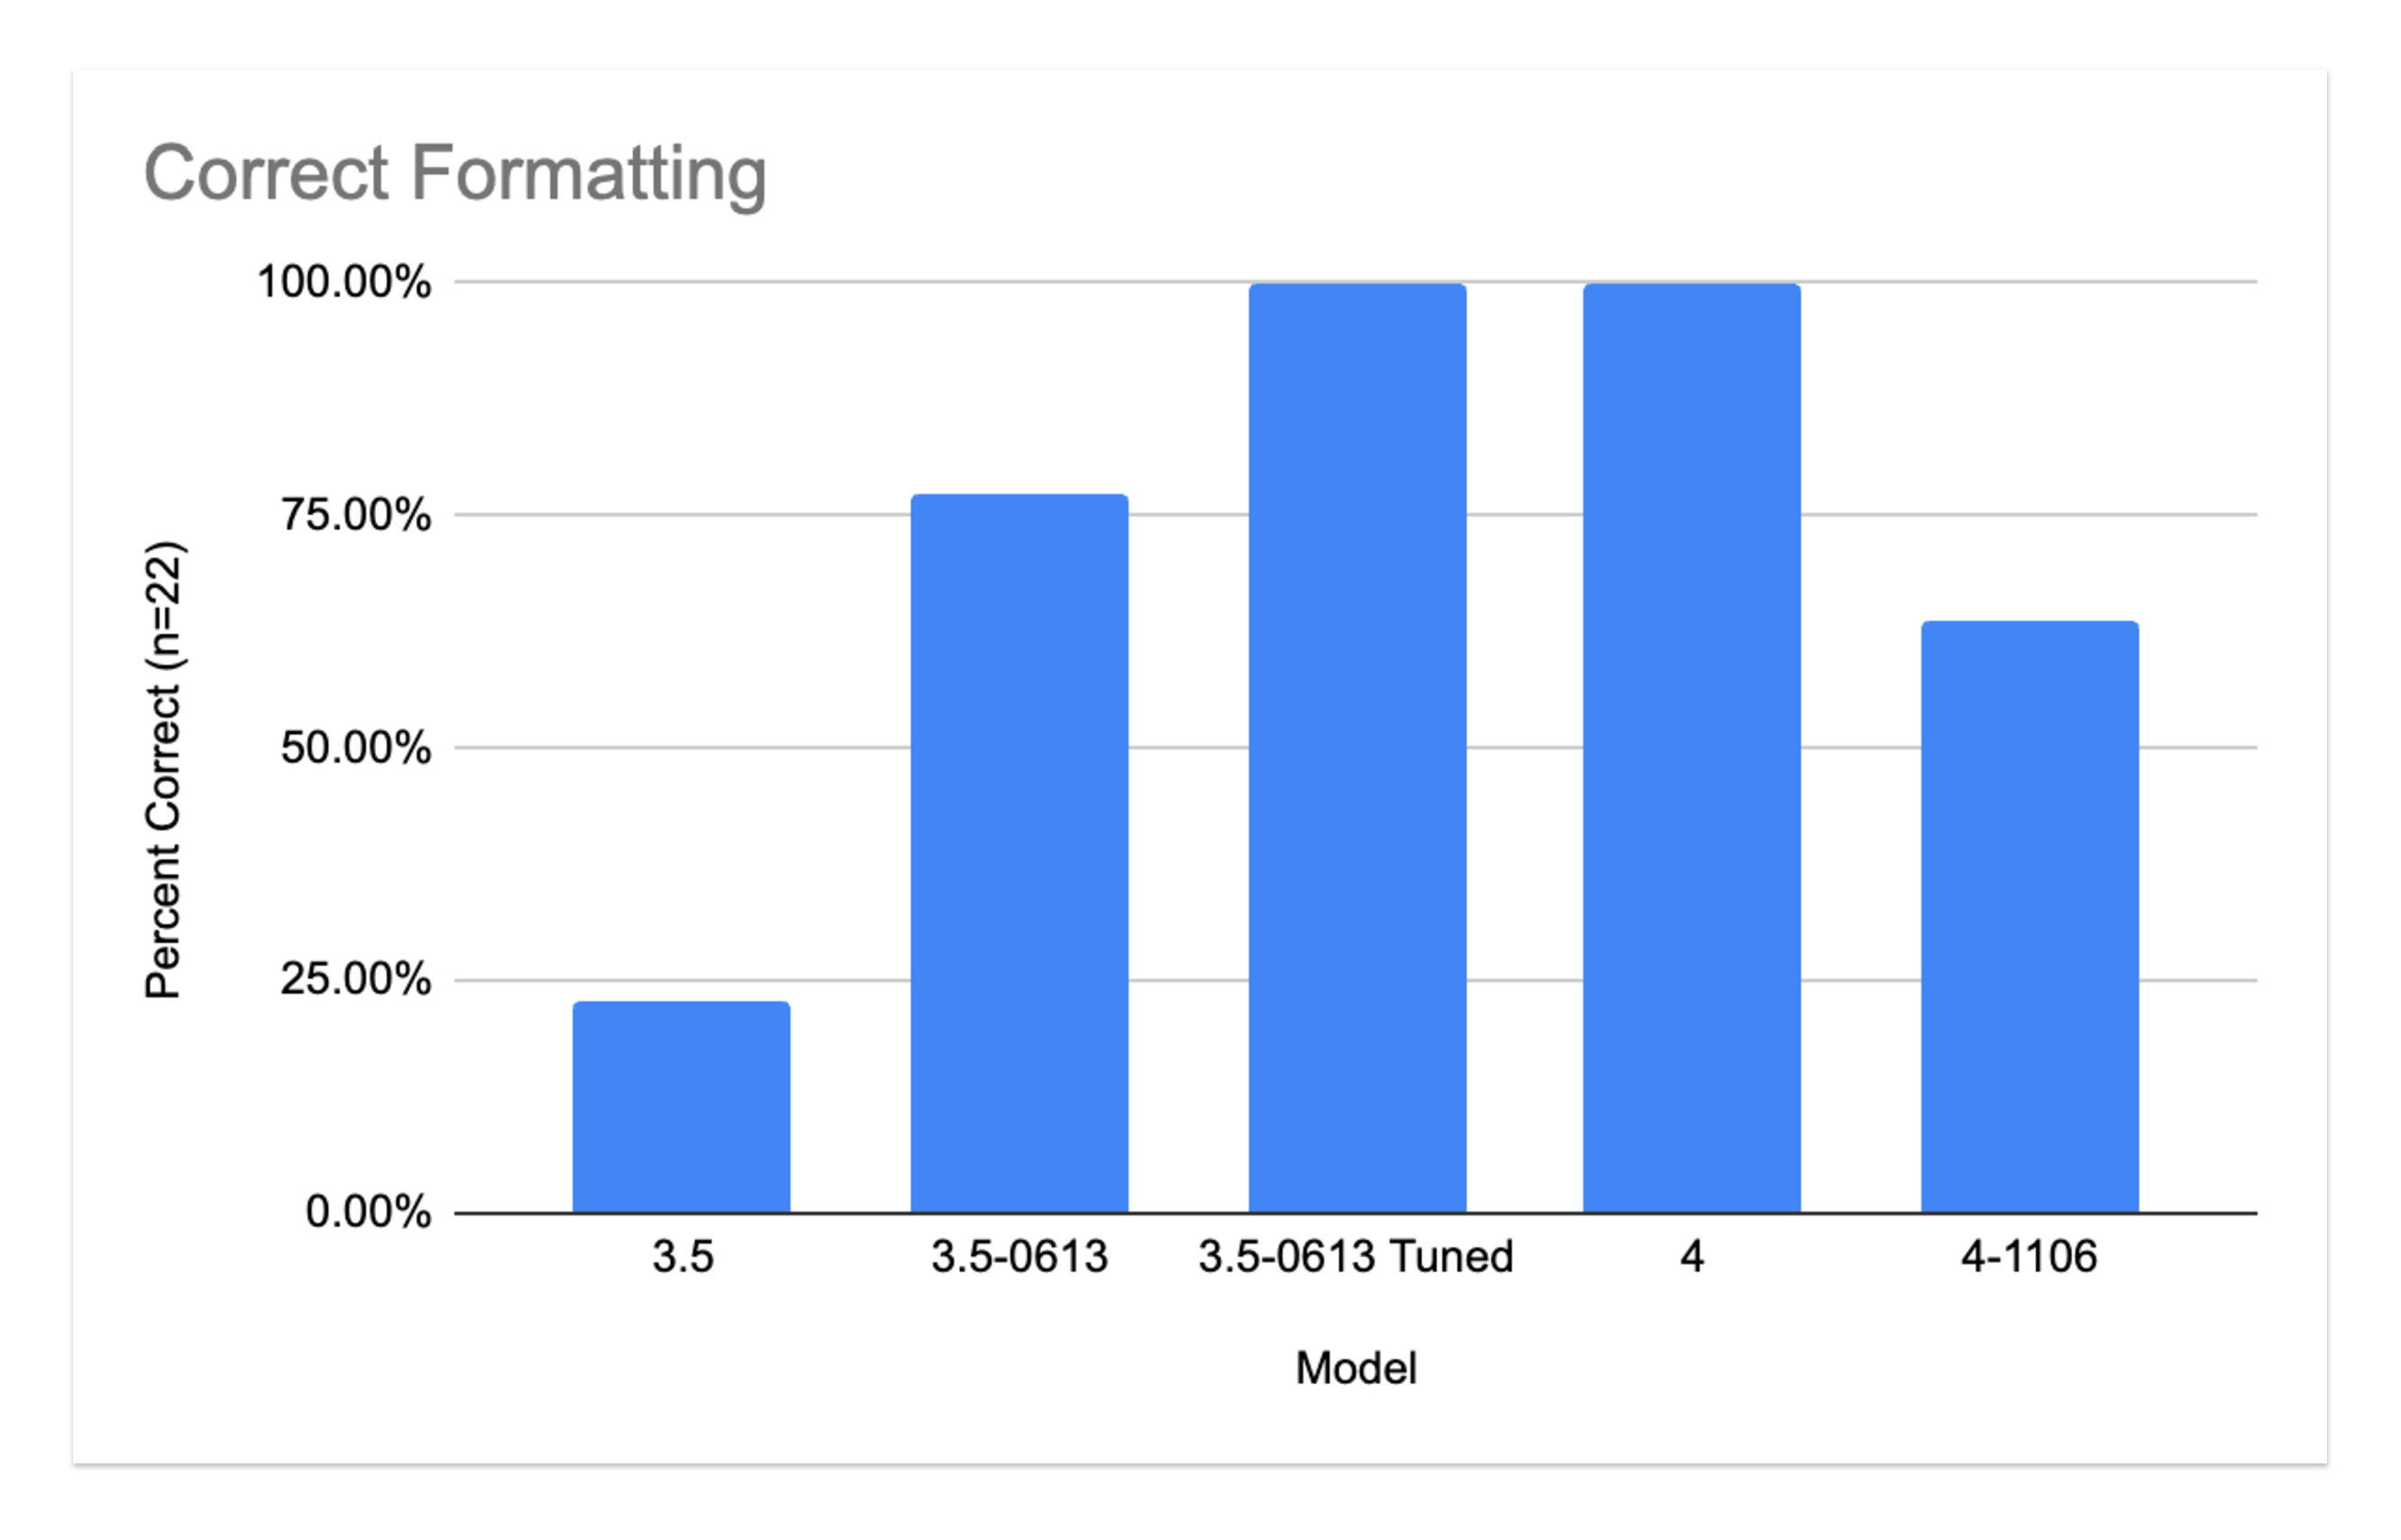
\includegraphics[scale=0.25]{../plots/2_correct_formatting.pdf}}
\caption{Percentage of correctly formatted outputs}
\end{figure}

Figure 3 shows the performance of each model at classifying the vulnerability type. You can see that the tuned model has a clear performance increase, moving up to gpt-4 levels of performance.\\

% 2_correct_categorization_of_vulnerability
\begin{figure}[htp] \centering{
  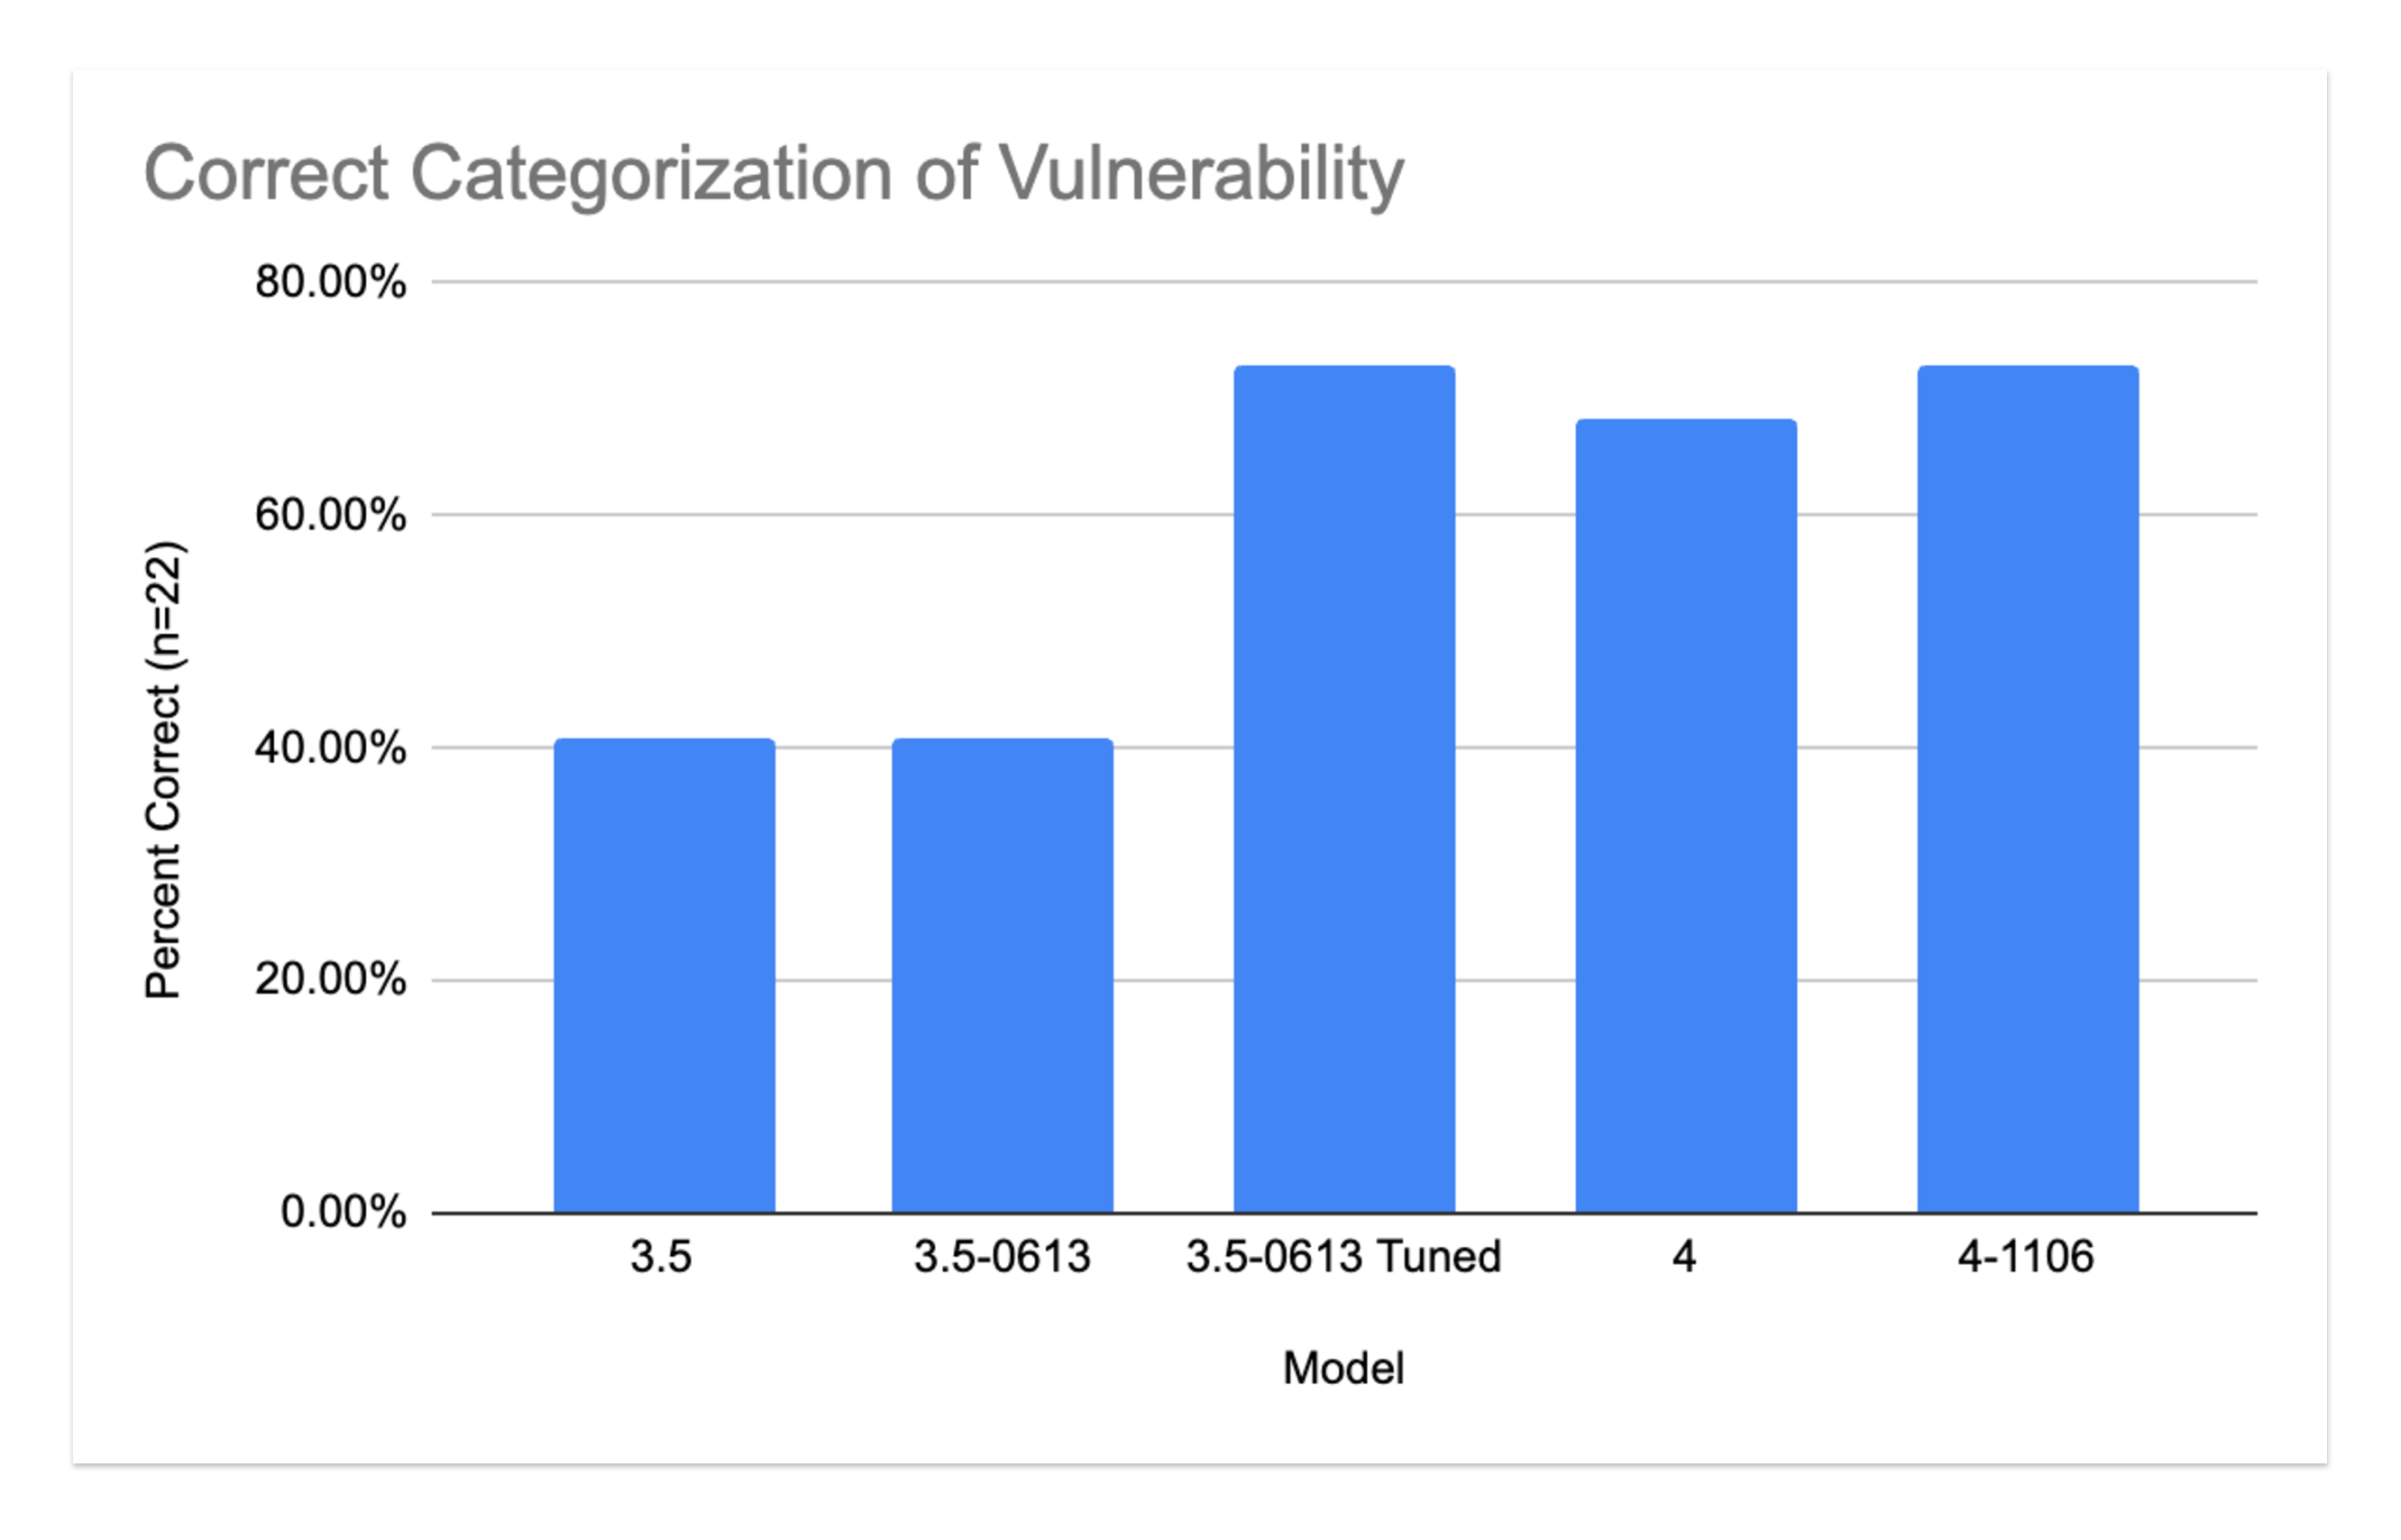
\includegraphics[scale=0.25]{../plots/1_correct_categorization_of_vulnerability.pdf}}
  \caption{Percentage of correctly categorized vulnerabilities}
  \end{figure}

Figure 4 shows the performance of each model at correctly classifying the vulnerability type and the source and sink locations. Here we can see a massive improvement in the tuned model's performance, even beyond gpt-4's current capabilities. 

This result is by far the most interesting in the data we collected. It suggests that the specific tuning of large language models can dramatically improve their static analysis performance. This result, however, needs to be verified on more data as this could be the result of overfitting on our training data.\\
  

% 3_correct_vulnerability_and_sink_source_locations.pdf
\begin{figure}[htp] \centering{
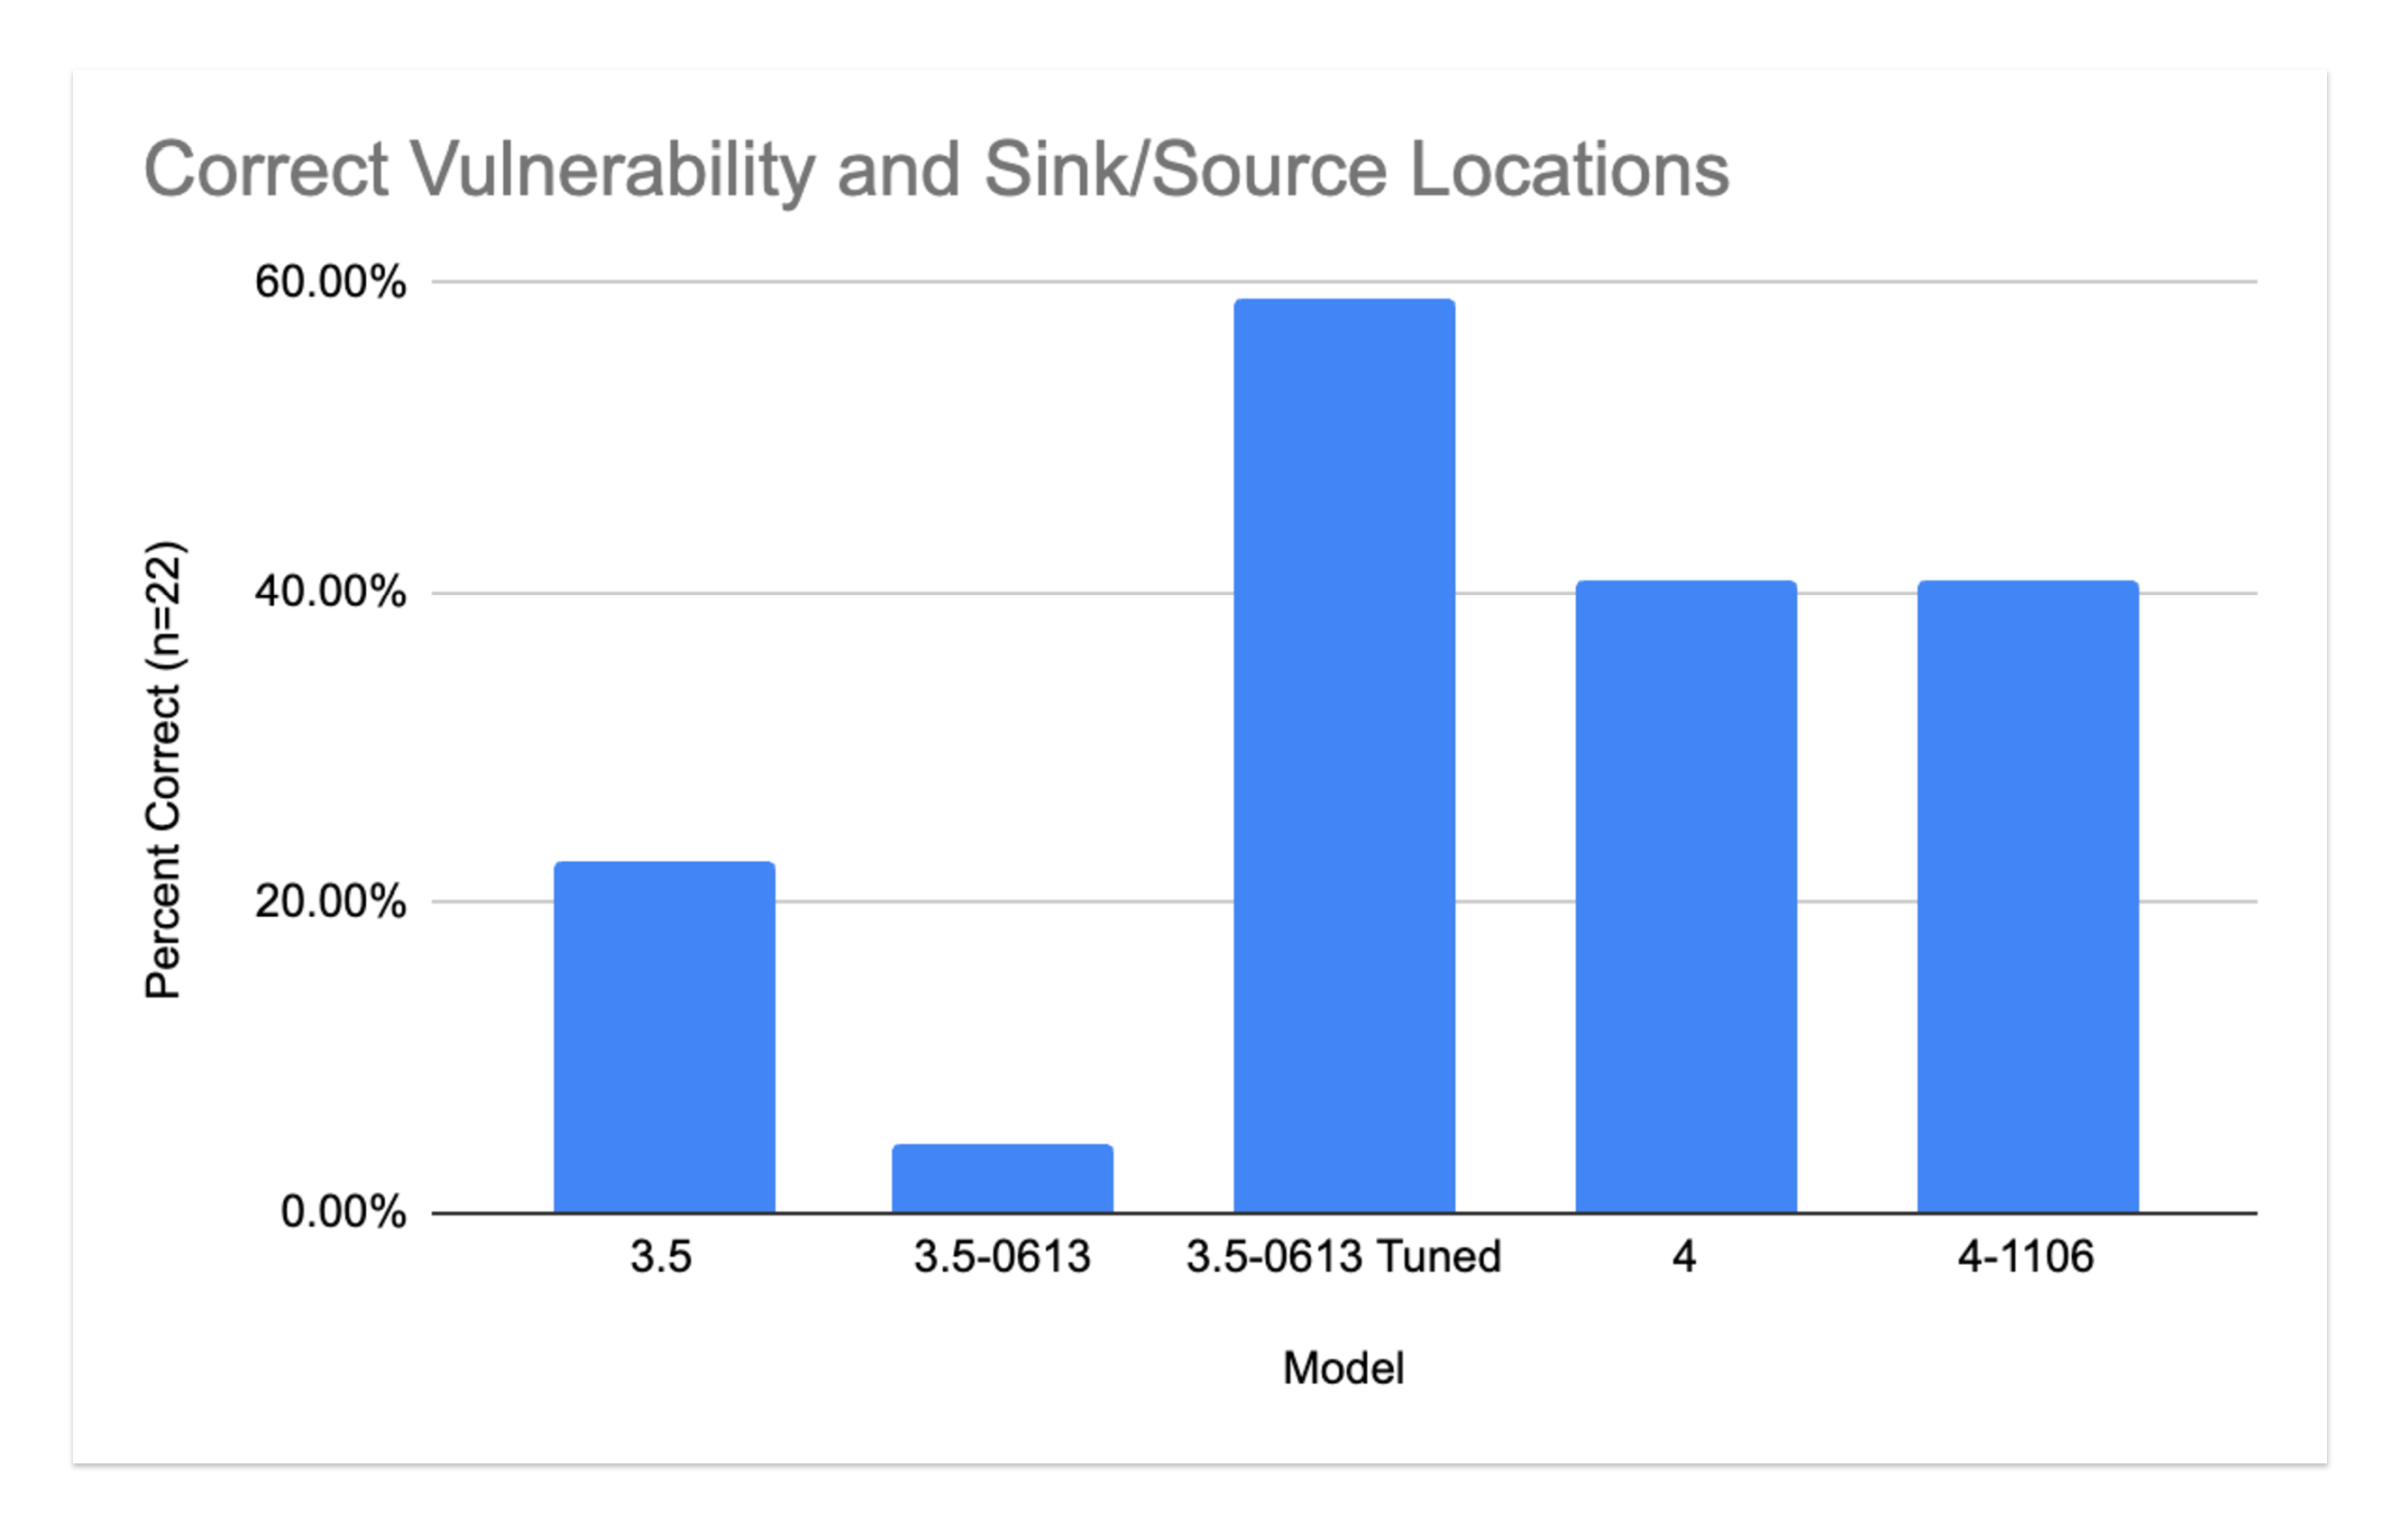
\includegraphics[scale=0.25]{../plots/3_correct_vulnerability_and_sink_source_locations.pdf}}
\caption{Percentage of correctly identified source and sink locations, as well as vulnerability categorization}
\end{figure}

Figure 5 shows the precision, recall, and f1 scores of each model. The score is calculated on whether or not the models predict the code is vulnerable or not. We see a large increase in recall with tuning without sacrificing precision. This suggests that tuning greatly increases the ability for large language models to recognize vulnerabilities.\\


% 4_precision_recall_and_F1_of_models
\begin{figure}[htp] \centering{
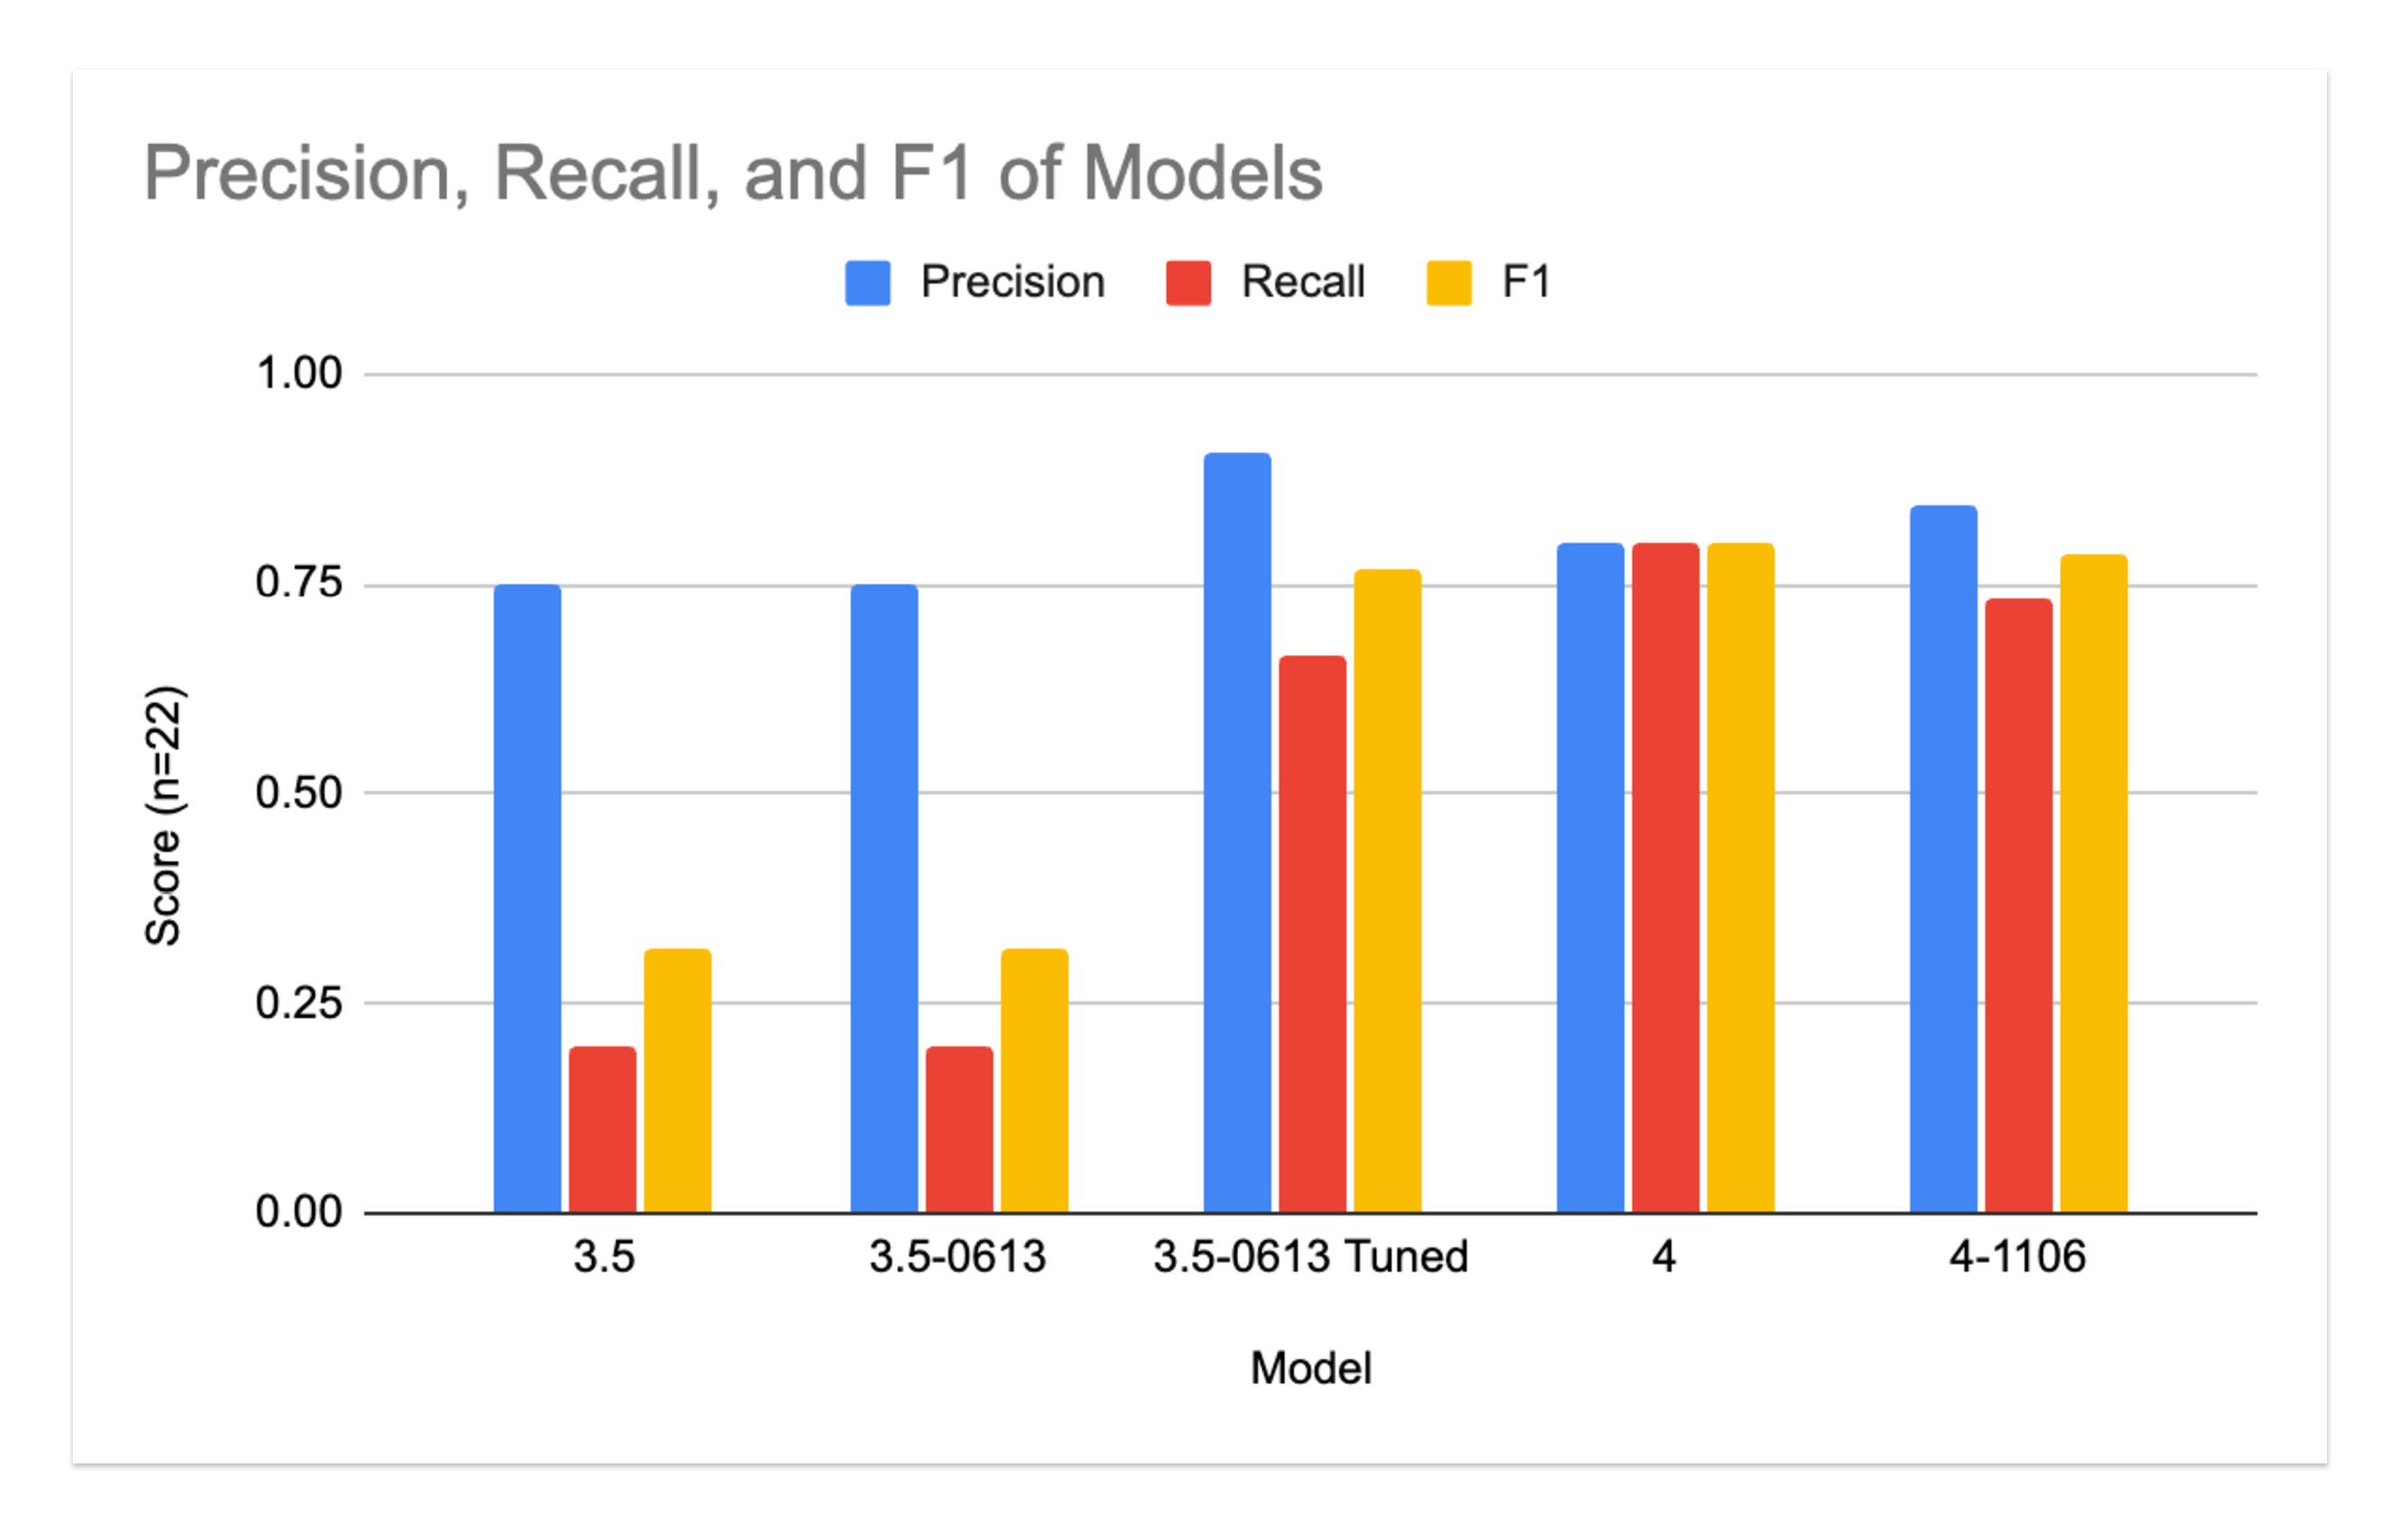
\includegraphics[scale=0.25]{../plots/4_precision_recall_and_F1_of_models.pdf}}
\caption{Precision, recall, and F1 scores for each model}
\end{figure}

Figure 6 shows the performance of each model on each classification of vulnerability. Of note here is that the untuned gpt-3.5 models perform well on identifying safe code because of a high false negative rate.

% 5_success_rate_for_each_vulnerability_type
\begin{figure}[htp] \centering{
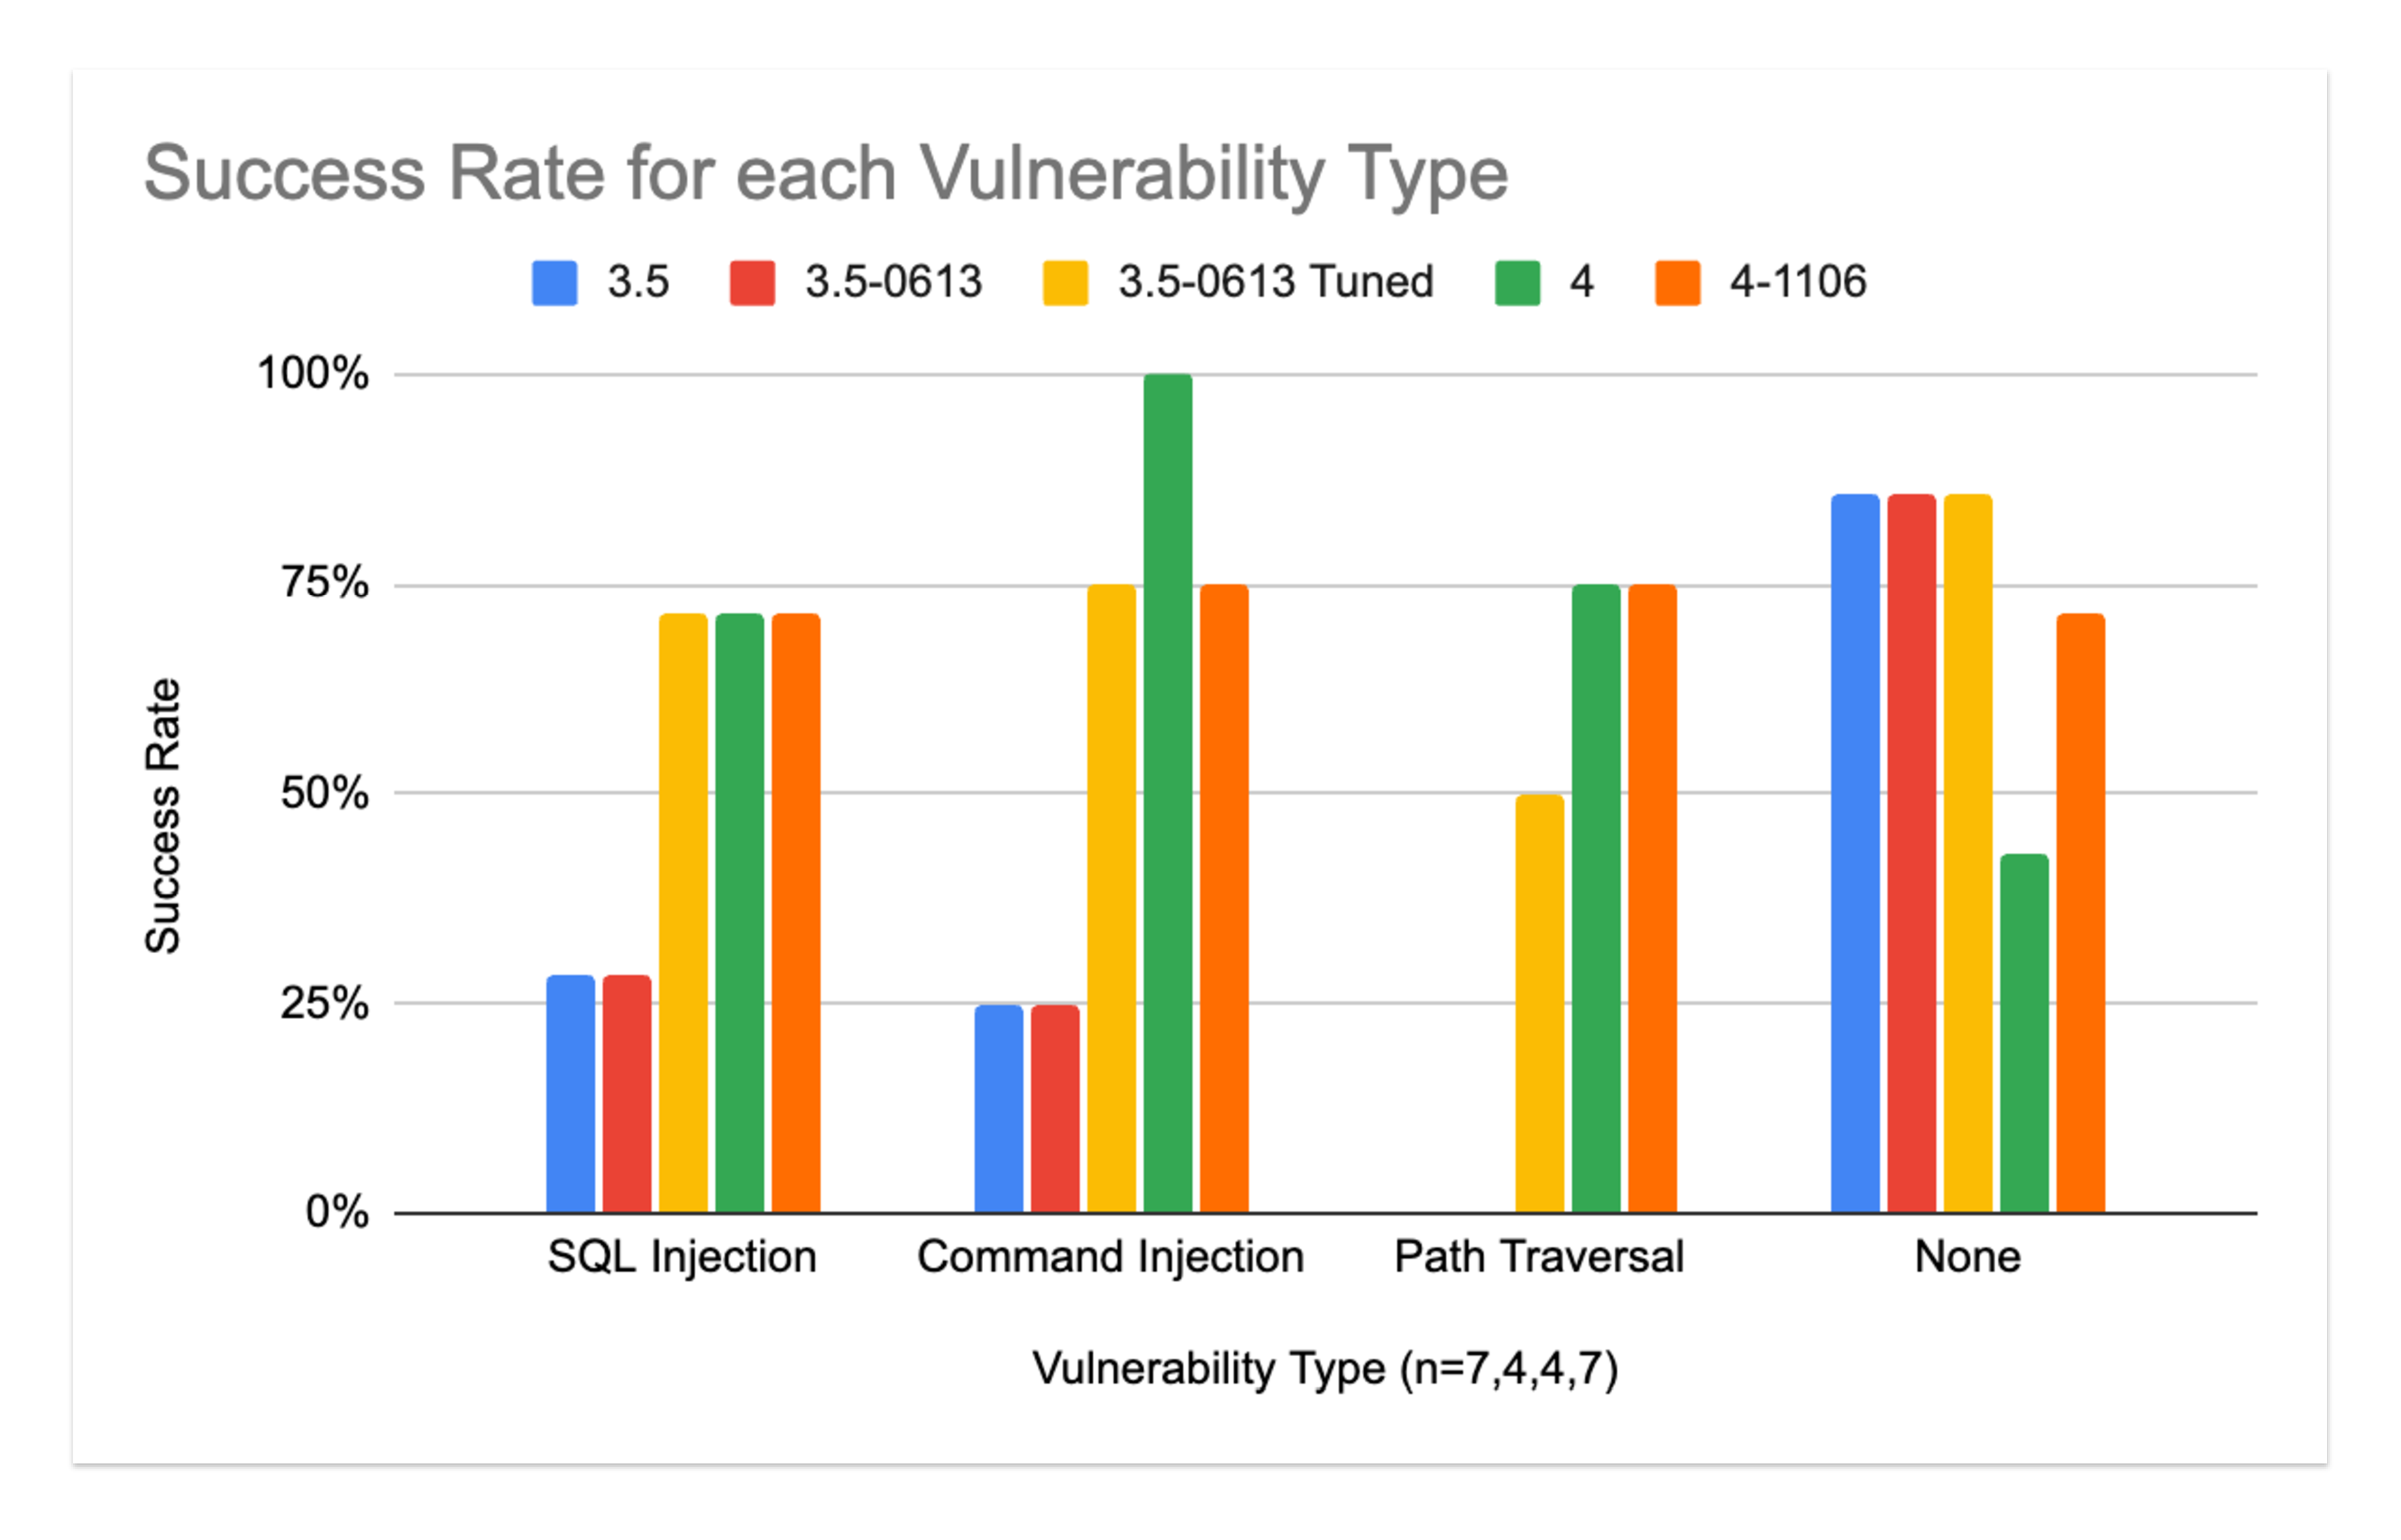
\includegraphics[scale=0.25]{../plots/5_success_rate_for_each_vulnerability_type.pdf}}
\caption{Success rate on each category of vulnerability}
\end{figure}
\section{Discussion}

\subsection{Inaccurate Identification and Communication of Line Location}
A major challenge we faced was the inaccurate identification and communication of line locations for sources and sinks in the code. This inaccuracy often occurred as ChatGPT sometimes overlooked empty lines or lines containing only comments. Precise line localization is vital for accurately pinpointing vulnerabilities in code. To mitigate this issue, we implemented a script to add line numbers to the start of each line in our dataset. This enhancement aims to improve the model's precision in pinpointing the exact lines where vulnerabilities begin (source) and where they could potentially lead to an exploit (sink). Accurate identification of these specific line locations is essential, as it enables developers to more effectively and efficiently address and rectify vulnerabilities.

\subsection{Time-Consuming and Less Diverse Dataset Creation}
The development of our dataset was a particularly time-intensive task, largely due to the detailed process necessary for ensuring that it included precise and relevant instances of SQL injection, command injection, and path traversal vulnerabilities. In the course of creating this dataset, we also faced challenges regarding its diversity. Here, diversity encompasses the variety of programming languages, coding styles, and the complexity levels of the vulnerabilities. This aspect is crucial because a dataset with a broader range of attributes could significantly enhance the model's ability to generalize its learning to a wider array of real-world scenarios.

To address these issues, we adopted a dual approach for dataset compilation. Half of our dataset was meticulously crafted in-house, ensuring a high level of detail and accuracy. The other half was sourced from the community, utilizing resources such as open-source repositories on GitHub, various technical blogs, and existing datasets. This hybrid approach was intended to strike a balance between precision and diversity, harnessing the breadth of community knowledge and insights while maintaining a strong focus on the quality and relevance of the data points.

\subsection{Number of Epochs Choosing Strategy}
In the process of model tuning, we faced the risk of underfitting and overfitting. We experimented with 1, 3, and 10 epochs for training and found that training for 3 epochs offered the best balance. Training for only one epoch led to underfitting, where the model was unable to learn enough from the dataset, while 10 epochs led to overfitting, where the model became too tailored to the training dataset and less effective at generalizing to new data. Finding the optimal number of epochs was crucial for achieving the best model performance.

\subsection{Dataset Splitting Strategy and Trade-off}
Determining the ideal division of our dataset presented a significant challenge, particularly given its relatively modest size, comprising only 25 SQL injection (SQLi), 15 path traversal, 15 command (cmd) injection, and 30 clean code cases. After careful consideration, we opted for a 60/10/30 split for training, validation, and testing. This allocation provided a substantial volume of data for training, ensuring that the model could learn effectively from a wide array of examples. However, it also meant that the validation set, which plays a critical role in model tuning during the training phase, was comparatively small.

The decision to allocate 30\% of our limited dataset to testing was strategic, driven by our aim to strengthen the robustness of our conclusions. Given the small number of cases, particularly in the categories of SQLi, path traversal, and cmd injection, it was imperative to have a more extensive testing dataset. This approach allowed us to evaluate the model's performance on a broader spectrum of unseen data, thereby providing a more comprehensive and reliable assessment of its capabilities in identifying and mitigating these specific types of vulnerabilities. The trade-off in reducing the size of the validation dataset was a necessary step to achieve this goal, ensuring that our findings were grounded in a solid and extensive testing process.

\subsection{Dataset Ground Truth Validity}
Ensuring the validity of the ground truth in our dataset was a crucial aspect of our project, given its direct impact on the model's learning efficacy. Ground truth, referring to the accuracy of data labeling, is essential for the model to learn and make correct predictions. Our team, comprised of just two members, faced inherent limitations, particularly in the breadth of expertise across various software vulnerabilities. To address this, we relied on peer reviews for validating our data. However, even with peer reviews, there remained the possibility of gaps in our dataset's comprehensiveness and precision, given the limited range of expertise among our reviewers.

In our labeling process, our team achieved a high consensus rate, agreeing on 76 out of 80 cases, which translates to a 95\% agreement rate. This high level of agreement underscores the rigorousness of our approach. However, the experience also highlighted the need for more diverse expertise in the creation and validation of such datasets.

In light of this, one of our primary objectives is to develop this dataset as an open-source project. The aim here is to invite participation from a broader community of experts and enthusiasts in software security. By opening up our dataset to the community, we hope to attract contributions from individuals with a wide range of expertise and perspectives. This collaborative approach is expected to significantly enhance the validity and reliability of our dataset. The community's input can help in identifying and correcting any overlooked vulnerabilities, thereby enriching the dataset and making it a more robust tool for training models in software vulnerability detection. This initiative is not only about expanding the dataset but also about fostering a collaborative environment where collective expertise contributes to advancing the field of AI in software security.

\section{Related Work}

In the study by Chow et al.\cite{Chow23}, the authors explored the use of several machine learning strategies to classify vulnerabilities and identify "unexpected" source and sink paths. In their research they found large language models to perform poorly when compared to other, more standard, models. We believe it would be interesting to explore their research again, this time with several fine tuned models, and evaluate the model's performance on their dataset and tasks.

\section{Conclusion}
Our intention with the project was to investigate the methods we can use to test and improve the performance of large language models performance on static analysis tasks. We believe this simple testing repository can help people investigate the efficacy of OpenAI's model tuning API as well as be a starting place for better datasets aimed at empirically investigating the performance of large language models.

The results of the paper suggest that tuning large language models for specific static analysis tasks may dramatically improve their performance. This result needs further verification though, as we have not yet demonstrated that the increased performance is not a result of overfitting. In future work we would like to test our tuned model on external datasets to see if the improvements are a result of insight or just data fitting. 


\bibliographystyle{ACM-Reference-Format}
\bibliography{b.bib}

\end{document}
\endinput